\documentclass{article}
\usepackage{ctex} % 添加中文支持包
\usepackage{geometry}
\geometry{margin=2.5cm}
\usepackage{graphicx}
\usepackage{mhchem}
\usepackage{amsmath}
\usepackage{booktabs}
\usepackage{hyperref}
\usepackage{graphicx}
\usepackage{float}
\usepackage{subcaption}
\usepackage{xcolor}

\title{Ex13}

\begin{document}
\newpage

\section{状态变量、输入}

状态变量45个\newline\newline
    1   {       'Uc\_DUT/CL'                   }\newline
    2   {       'Uc\_DUT/Cs'                   }\newline
    3   {       'Uc\_DUT/Cs1'                  }\newline
    4   {       'Uc\_DUT/Cs2'                  }\newline
    5   {       'Uc\_DUT/Cs3'                  }\newline
    \textcolor{red}{6   {       'Uc\_DUT/Ct'                   }}\newline
    7   {       'Il\_DUT/DUT/Lon'              }\newline
    \textcolor{red}{8   {       'Uc\_DUT/DUT/Series RLC Branch'}}\newline
    9   {       'Il\_DUT/L1'                   }\newline
    10  {       'Il\_DUT/L2'                  }\newline
    \textcolor{red}{11  {       'Il\_DUT/L3'                  }}\newline
    \textcolor{red}{12  {       'Il\_DUT/L4'                  }}\newline
    \textcolor{red}{13  {       'Il\_DUT/L5'                  }}\newline
    \textcolor{red}{14  {       'Il\_DUT/Va1/Lon'             }}\newline
    15  {       'Uc\_DUT/Va1/Series RLC Branch'}\newline
    \textcolor{red}{16  {       'Il\_DUT/Va2/Lon'             }}\newline
    17  {       'Uc\_DUT/Va2/Series RLC Branch'}\newline
    \textcolor{red}{18  {       'Il\_DUT/Va3/Lon'             }}\newline
    19  {       'Uc\_DUT/Va3/Series RLC Branch'}\newline
    \textcolor{red}{20  {       'Il\_DUT/Va4/Lon'             }}\newline
    21  {       'Uc\_DUT/Va4/Series RLC Branch'}\newline
    \textcolor{red}{22  {       'Il\_DUT/Va5/Lon'             }}\newline
    23  {       'Uc\_DUT/Va5/Series RLC Branch'}\newline
    \textcolor{red}{24  {       'Il\_DUT/Vc1/Lon'              }}\newline
    25  {       'Uc\_DUT/Vc1/Series RLC Branch'}\newline
    \textcolor{red}{26  {       'Il\_DUT/Vc2/Lon'              }}\newline
    27  {       'Uc\_DUT/Vc2/Series RLC Branch'}\newline
    \textcolor{red}{28  {       'Il\_DUT/Vc3/Lon'              }}\newline
    29  {       'Uc\_DUT/Vc3/Series RLC Branch'}\newline
    \textcolor{red}{30  {       'Il\_DUT/Vc4/Lon'              }}\newline
    31  {       'Uc\_DUT/Vc4/Series RLC Branch'}\newline
    \textcolor{red}{32  {       'Il\_DUT/Vc5/Lon'              }}\newline
    33  {       'Uc\_DUT/Vc5/Series RLC Branch'}\newline
    34  {       'Il\_Series RLC Branch2'       }\newline
    35  {       'Il\_Series RLC Branch3'       }\newline
    36  {       'Uc\_T1/C'                     }\newline
    \textcolor{red}{37  {       'Il\_T1/Lon'                   }}\newline
    38  {       'Uc\_T2/C'                     }\newline
    \textcolor{red}{39  {       'Il\_T2/Lon'                   }}\newline
    40  {       'Uc\_T3/C'                     }\newline
    \textcolor{red}{41  {       'Il\_T3/Lon'                   }}\newline
    42  {       'Uc\_T4/C'                     }\newline
    \textcolor{red}{43  {       'Il\_T4/Lon'                   }}\newline
    44  {       'Uc\_T6/C'                     }\newline
    \textcolor{red}{45  {       'Il\_T6/Lon'                   }}\newline
    {       'Il\_Series RLC Branch1*'      }\newline


\indent 输入变量23个（24:39均不使用）\newline\newline
    1   {      'I\_DUT/Ideal Switch'         }\newline
    2   {      'I\_DUT/DUT/T'                }\newline
    3   {      'I\_DUT/Va1/T'                }\newline
    4   {      'I\_DUT/Va2/T'                }\newline
    5   {      'I\_DUT/Va3/T'                }\newline
    6   {      'I\_DUT/Va4/T'                }\newline
    7   {      'I\_DUT/Va5/T'                }\newline
    8   {      'I\_DUT/Vc1/T'                }\newline
    9   {      'I\_DUT/Vc2/T'                }\newline
    10  {      'I\_DUT/Vc3/T'                }\newline
    11  {      'I\_DUT/Vc4/T'                }\newline
    12  {      'I\_DUT/Vc5/T'                }\newline
    13  {      'I\_T1/T'                     }\newline
    14  {      'I\_T2/T'                     }\newline
    15  {      'I\_T3/T'                     }\newline
    16  {      'I\_T4/T'                     }\newline
    17  {      'I\_T6/T'                     }\newline
    18  {      'U\_DUT/DC Voltage Source'    }\newline
    19  {      'U\_AC Voltage Source'        }\newline
    20  {      'U\_AC Voltage Source1'       }\newline
    21  {      'U\_AC Voltage Source2'       }\newline
    22  {      'U\_DUT/AC Voltage Source1'   }\newline
    23  {      'I\_Controlled Current Source'}\newline
    24  {      'U\_Vf: DUT/DUT/T'            }\newline
    25  {      'U\_Vf: DUT/Va1/T'            }\newline
    26  {      'U\_Vf: DUT/Va2/T'            }\newline
    27  {      'U\_Vf: DUT/Va3/T'            }\newline
    28  {      'U\_Vf: DUT/Va4/T'            }\newline
    29  {      'U\_Vf: DUT/Va5/T'            }\newline
    30  {      'U\_Vf: DUT/Vc1/T'            }\newline
    31  {      'U\_Vf: DUT/Vc2/T'            }\newline
    32  {      'U\_Vf: DUT/Vc3/T'            }\newline
    33  {      'U\_Vf: DUT/Vc4/T'            }\newline
    34  {      'U\_Vf: DUT/Vc5/T'            }\newline
    35  {      'U\_Vf: T1/T'                 }\newline
    36  {      'U\_Vf: T2/T'                 }\newline
    37  {      'U\_Vf: T3/T'                 }\newline
    38  {      'U\_Vf: T4/T'                 }\newline
    39  {      'U\_Vf: T6/T'                 }\newline

\newpage
\section{转换矩阵}
\begin{figure}[H] % 使用[H]选项将图片固定在当前位置
    \centering
    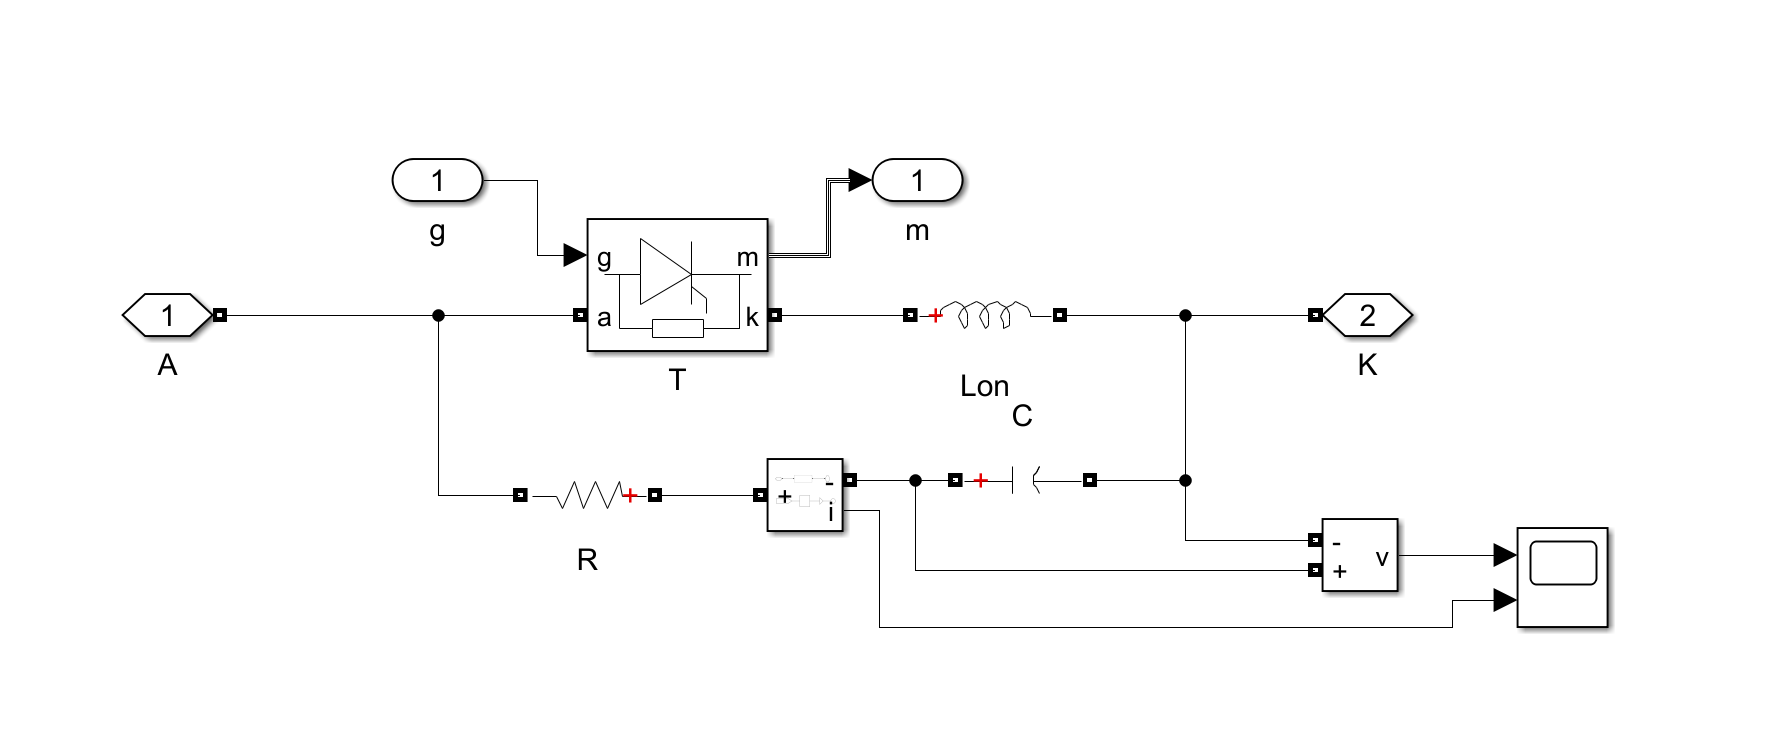
\includegraphics[width=0.8\textwidth]{T1_sim.png}
    \caption{sim模型T1, T2, T3, T4, T6, Va1, Va2, Va3, Va4, Va5, Vc1, Vc2, Vc3, Vc4, Vc5}
    \label{fig:motor_structures}
\end{figure}
\begin{figure}[H] % 使用[H]选项将图片固定在当前位置
    \centering
    
\includegraphics[width=0.8\textwidth]{T1.png}
    \caption{等效电路T1, T2, T3, T4, T6, Va1, Va2, Va3, Va4, Va5, Vc1, Vc2, Vc3, Vc4, Vc5}
    \label{fig:motor_structures}
\end{figure}

\indent state=1 时：\newline
\indent $(\frac{1}{Ron} + \frac{1}{Rs}) \times v_{d} = i_{L} - \frac{Vf}{Rs}$\newline
\indent $i_{d} = (\frac{1}{Ron}) \times v_{d}$\newline

\indent state=0 时：\newline
\indent $(\frac{1}{Rs}) \times v_{d} = i_{L} - \frac{Vf}{Rs}$\newline
\indent $i_{d} = 0$\newline
\begin{figure}[H] % 使用[H]选项将图片固定在当前位置
    \centering
    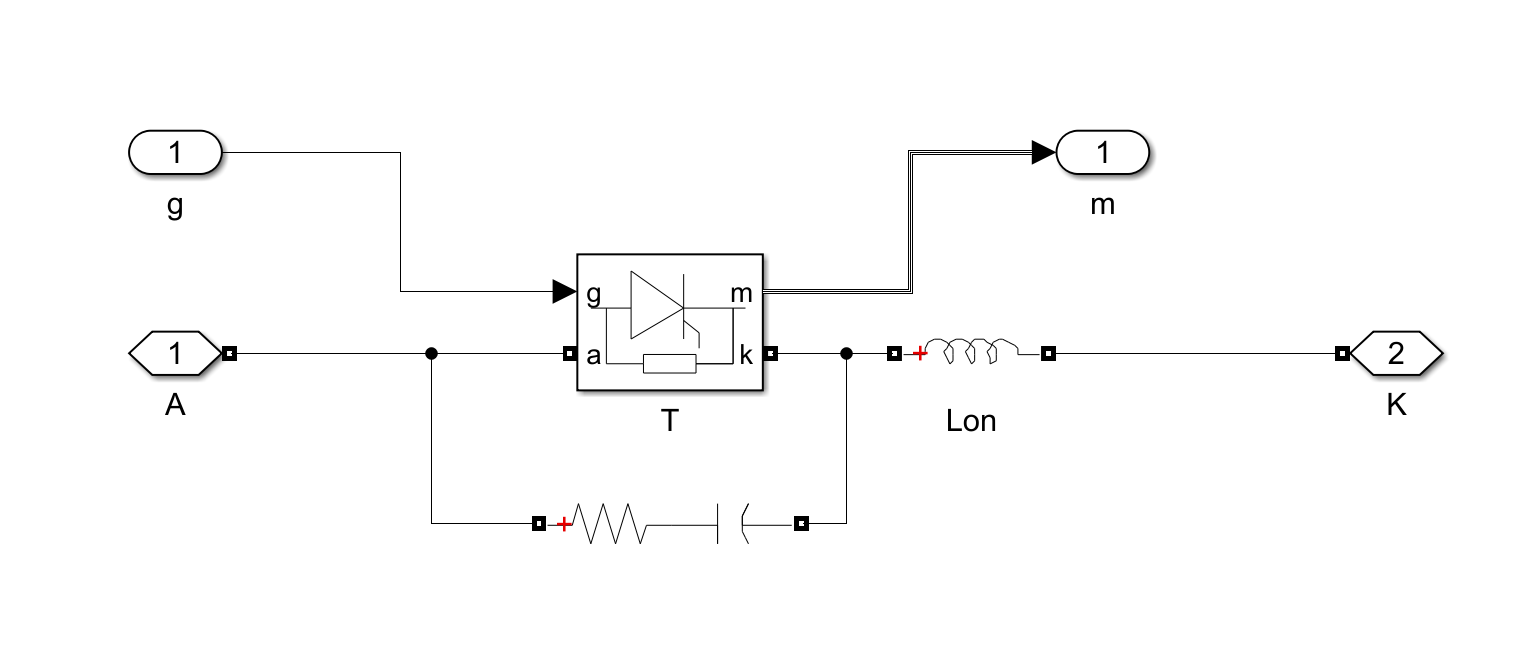
\includegraphics[width=0.8\textwidth]{DUT_sim.png}
    \caption{sim模型DUT}
    \label{fig:motor_structures}
\end{figure}

\begin{figure}[H] % 使用[H]选项将图片固定在当前位置
    \centering
    
\includegraphics[width=0.8\textwidth]{DUT.png}
    \caption{等效电路DUT}
    \label{fig:motor_structures}
\end{figure}

\indent state=1 时：\newline
\indent  $v_{d} = V_{RLC} - Vf$\newline
\indent $i_{d} = (\frac{1}{Ron}) \times v_{d}$\newline

\indent state=0 时：\newline
\indent $ v_{d} = V_{RLC} - Vf$\newline
\indent $i_{d} = 0$\newline


\begin{figure}[H] % 使用[H]选项将图片固定在当前位置
    \centering
    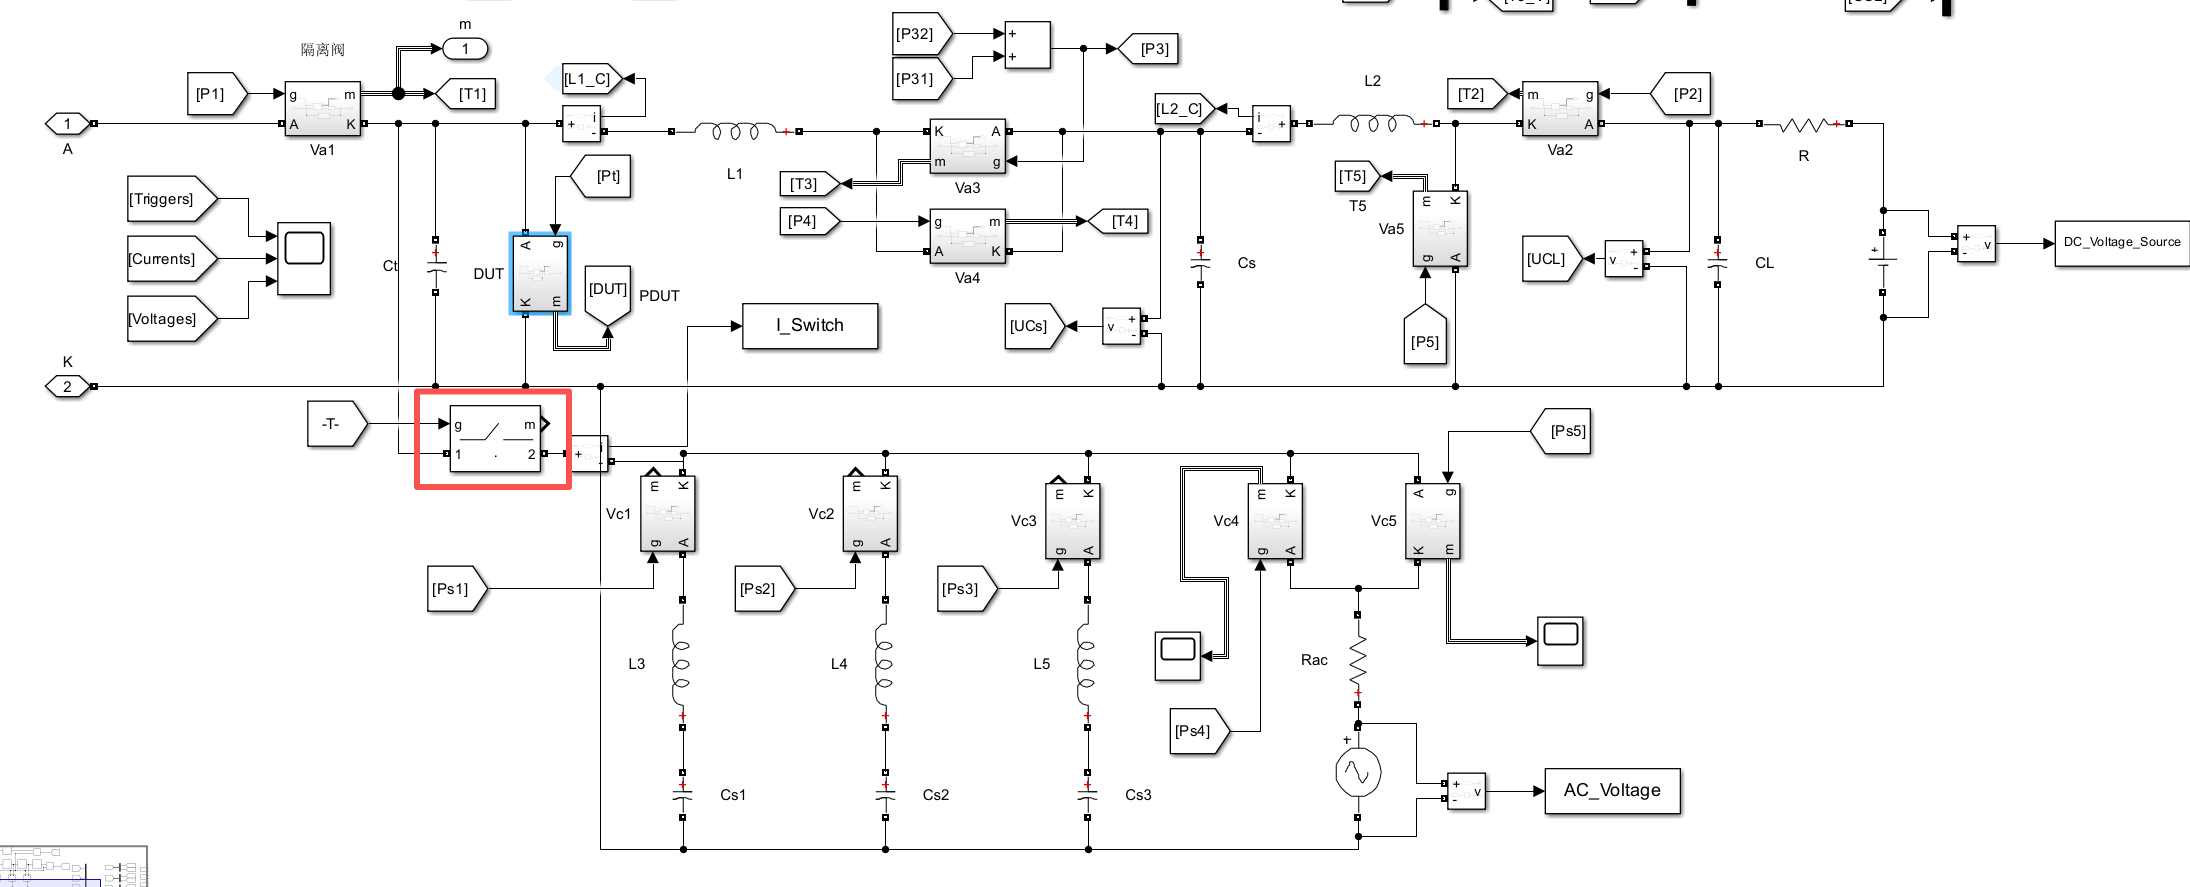
\includegraphics[width=1\textwidth]{Switch_sim.png}
    \caption{sim模型Ideal Switch}
    \label{fig:motor_structures}
\end{figure}

\begin{figure}[H] % 使用[H]选项将图片固定在当前位置
    \centering
    
\includegraphics[width=0.8\textwidth]{Switch.png}
    \caption{等效电路Ideal Switch}
    \label{fig:motor_structures}
\end{figure}

\indent state=1 时：\newline
\indent $(1 + \frac{Rac}{Ron}) \times v_{d} = V_{ct} + V_{c4} - Rac \times i_{L3} - Rac \times i_{L4} - Rac \times i_{L5} - V_{ac}$\newline
\indent $i_{d} = (\frac{1}{Ron}) \times v_{d}$\newline

\indent state=0 时：\newline
\indent $v_{d} = V_{ct} + V_{c4} - Rac \times i_{L3} - Rac \times i_{L4} - Rac \times i_{L5} - V_{ac}$\newline
\indent $i_{d} = 0$\newline

\indent 其中$V_{ac}$是已知源，所以从状态变量到输入的转换公式为 $A*v = B*x + b_{vf} + u_{vf}*u$\newline

\newpage
\section{仿真结果}

\indent 部分状态变量能够较好收敛。
\begin{figure}[H] % 使用[H]选项将图片固定在当前位置
    \centering
    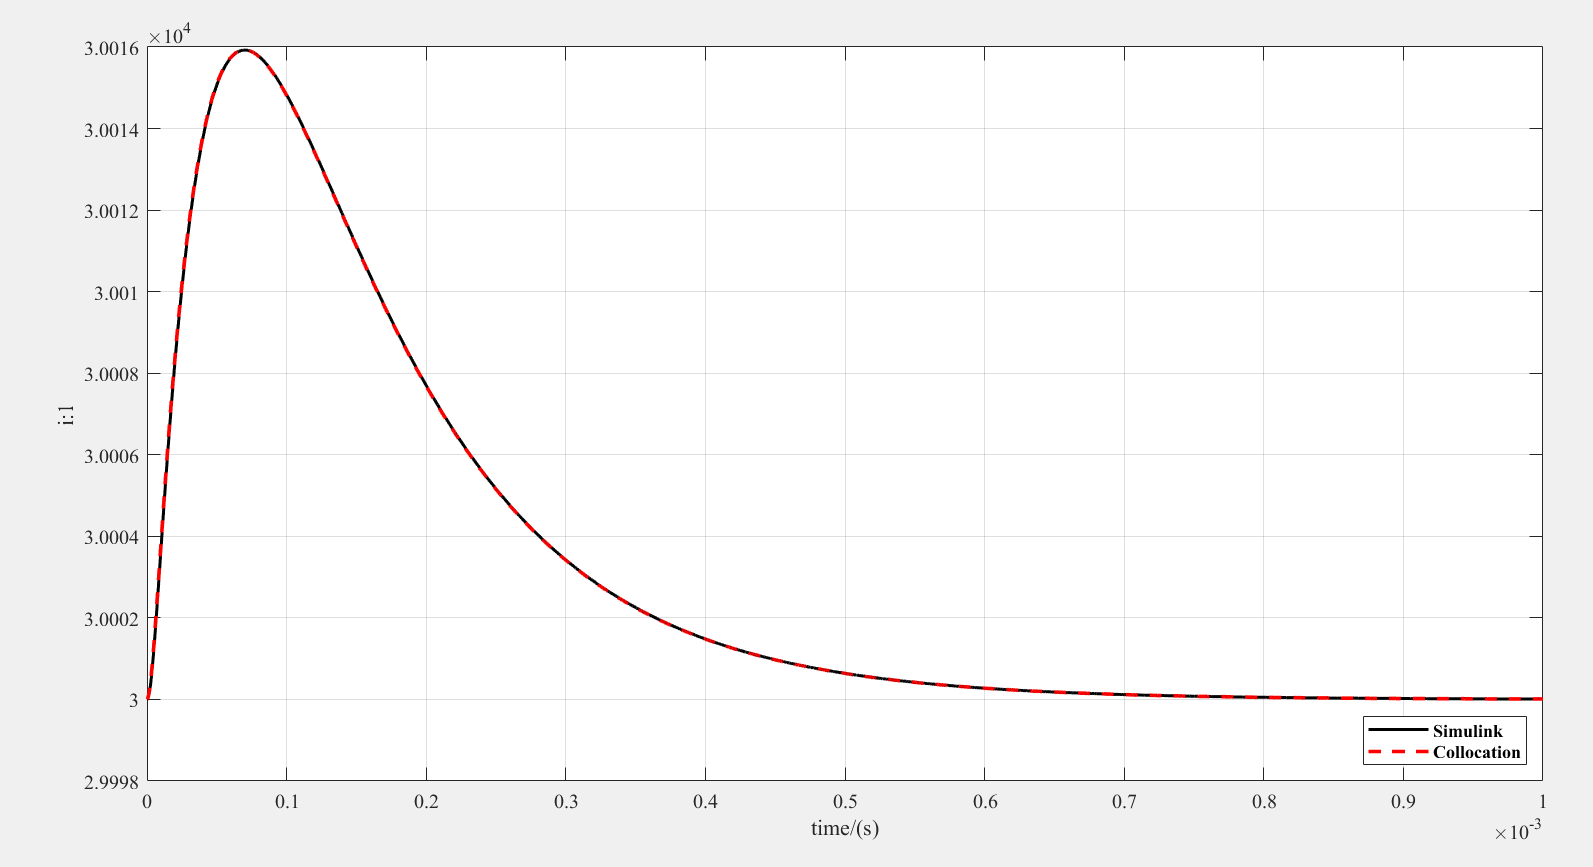
\includegraphics[width=0.8\textwidth]{DUT_CL.png}
    \caption{DUT-CL}
    \label{fig:motor_structures}
\end{figure}
\begin{figure}[H] % 使用[H]选项将图片固定在当前位置
    \centering
    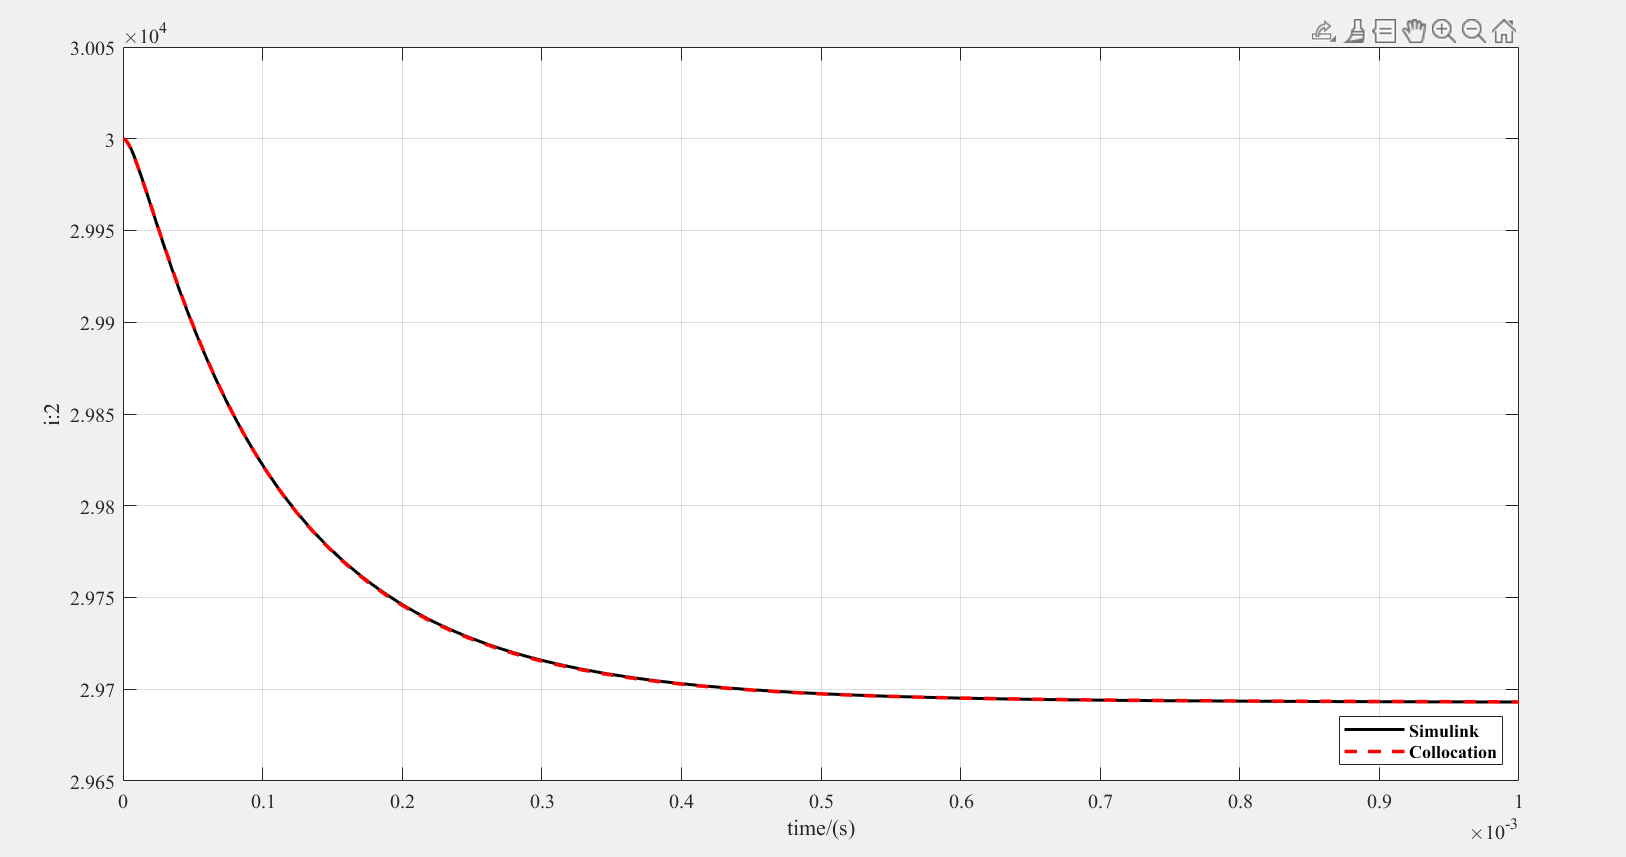
\includegraphics[width=0.8\textwidth]{DUT_Cs.png}
    \caption{DUT-Cs}
    \label{fig:motor_structures}
\end{figure}

\indent 部分状态变量难以收敛
\begin{figure}[H] % 使用[H]选项将图片固定在当前位置
    \centering
    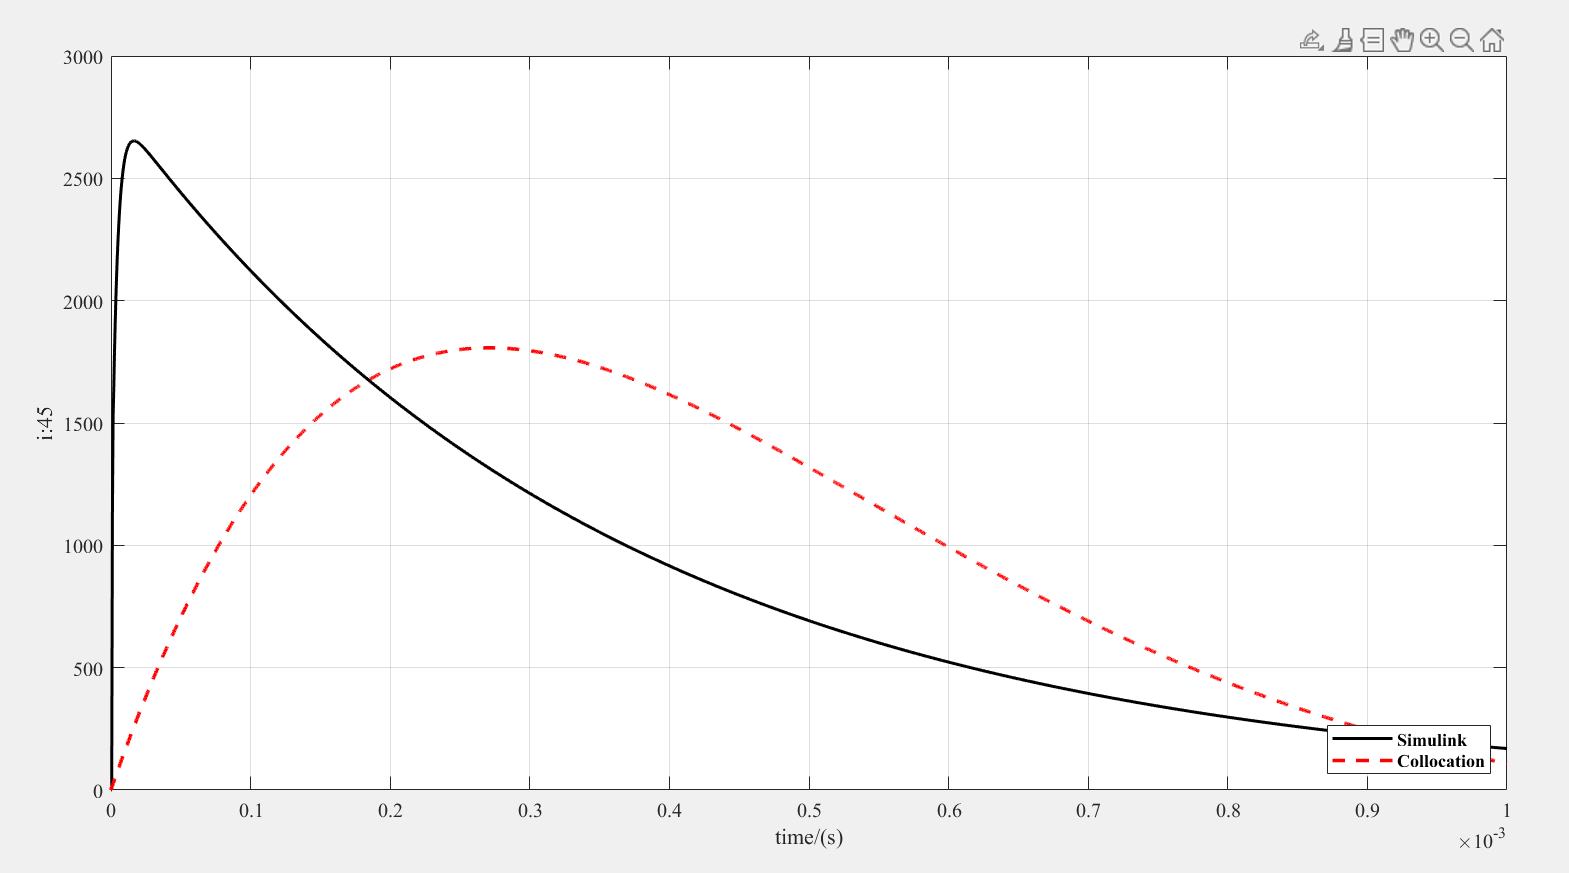
\includegraphics[width=0.8\textwidth]{45.png}
    \caption{T6-IL (kmax=100, t=[0,1e-3])}
    \label{fig:motor_structures}
\end{figure}

\begin{figure}[H] % 使用[H]选项将图片固定在当前位置
    \centering
    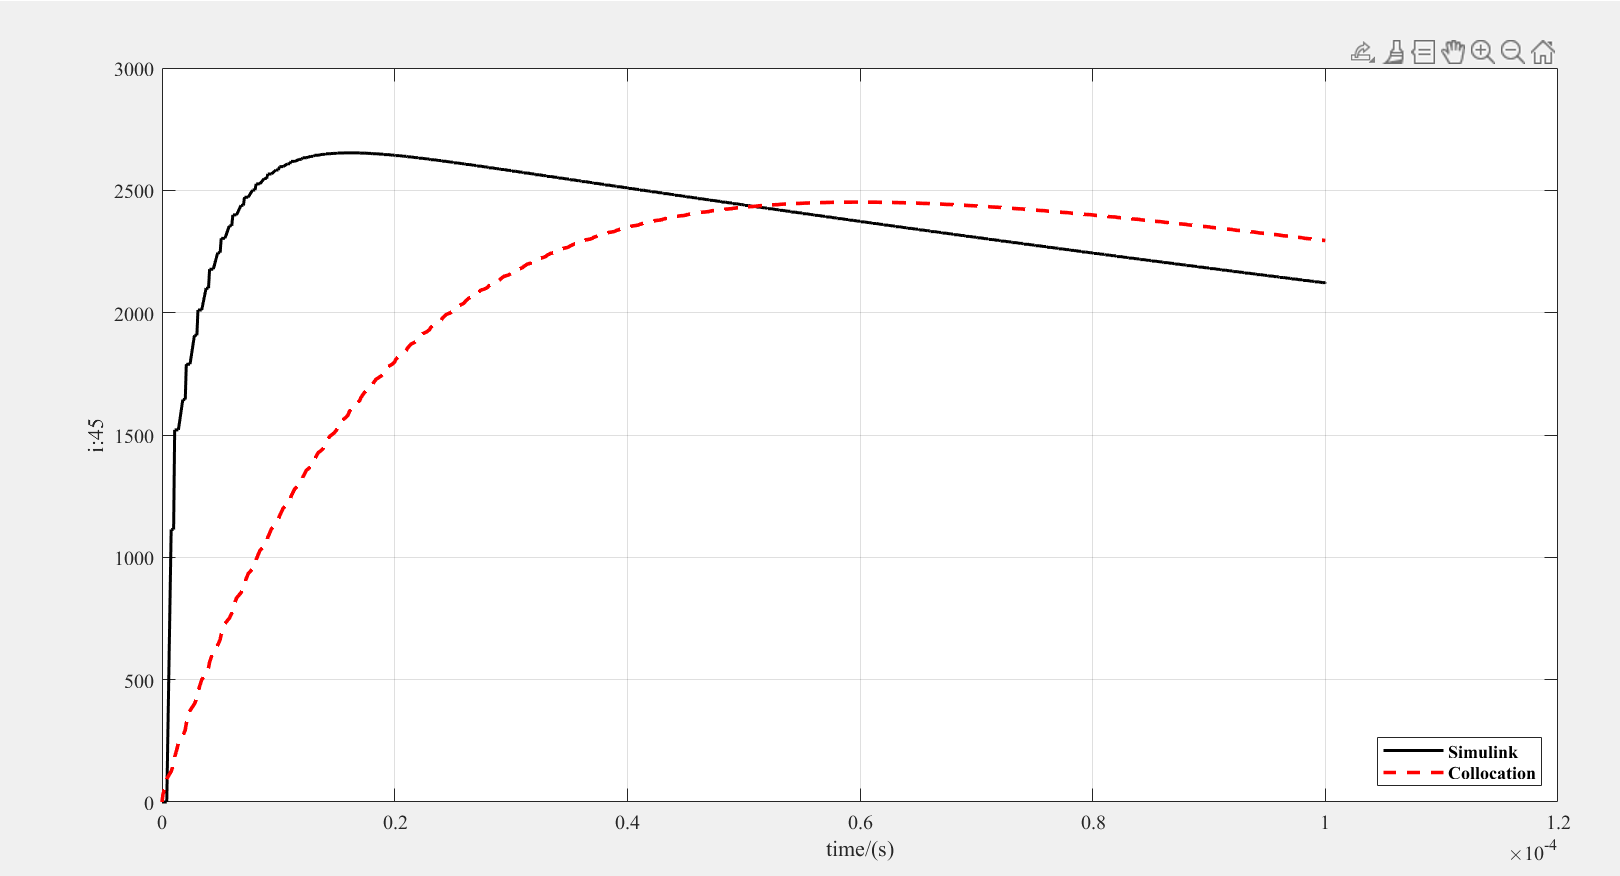
\includegraphics[width=0.8\textwidth]{45_1000.png}
    \caption{T6-IL (kmax=1000, t=[0,1e-4])}
    \label{fig:motor_structures}
\end{figure}


\indent Collocation运行时间(kmax=1000): \newline
\indent \text{Collocation() Total Execution Time: 95.4388 s}
\indent \text{Collocation() Total Execution Steps: 101 }\newline
\indent \text{Collocation\_onestep():  95.4328 s}
\indent \text{save\_results():  0.0012 s}

\begin{figure}[H] % 使用[H]选项将图片固定在当前位置
    \centering
    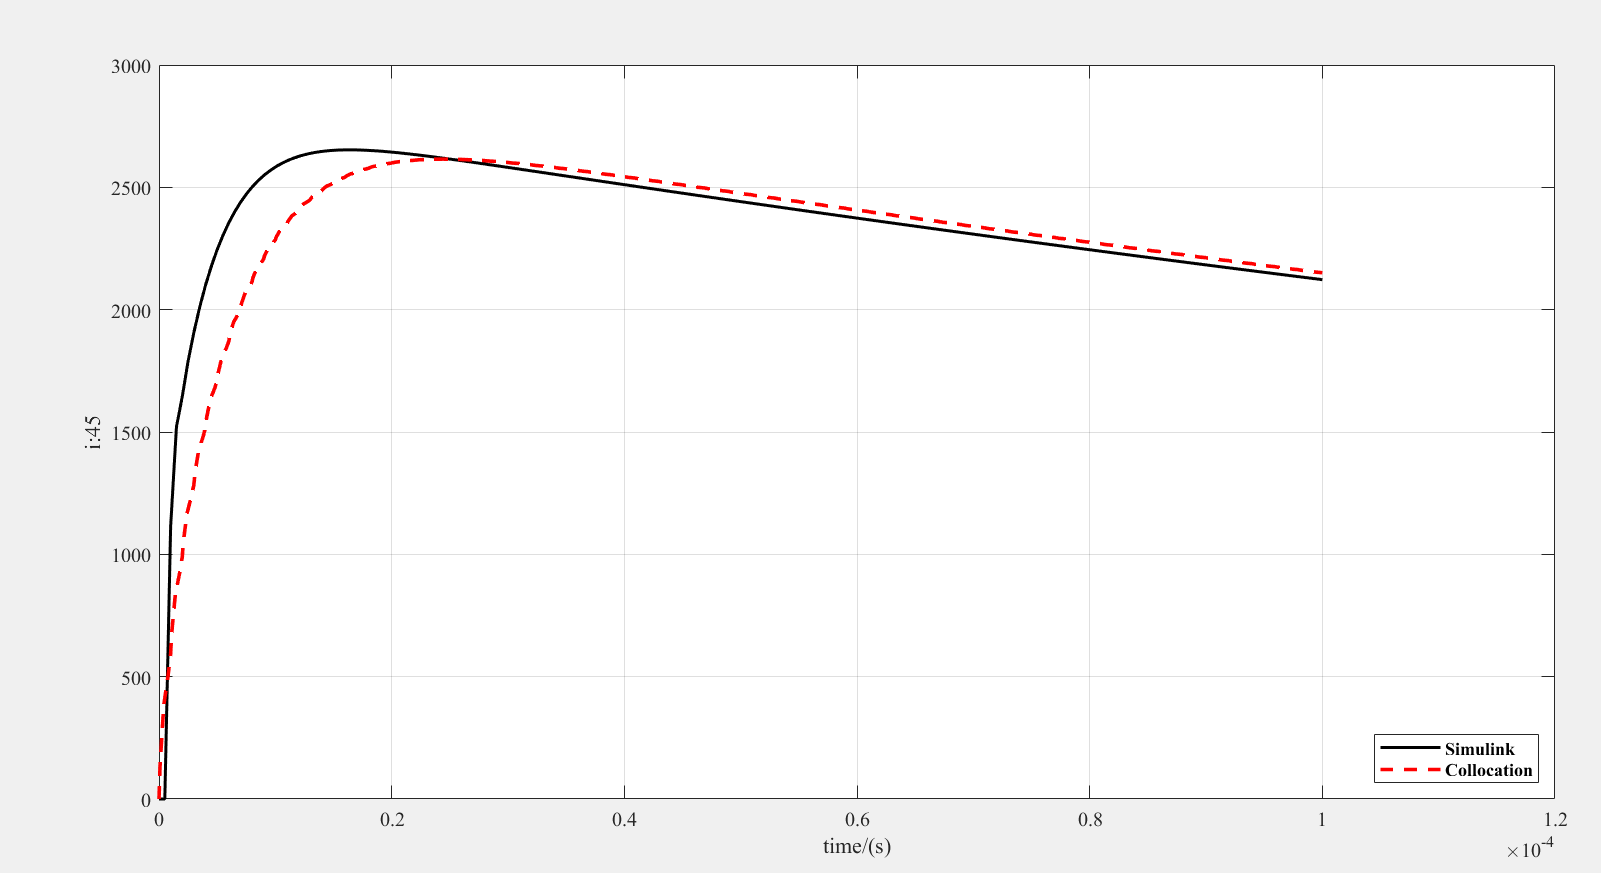
\includegraphics[width=0.8\textwidth]{45_5000.png}
    \caption{T6-IL (kmax=5000, t=[0,1e-4])}
    \label{fig:motor_structures}
\end{figure}


\begin{figure}[H] % 使用[H]选项将图片固定在当前位置
    \centering
    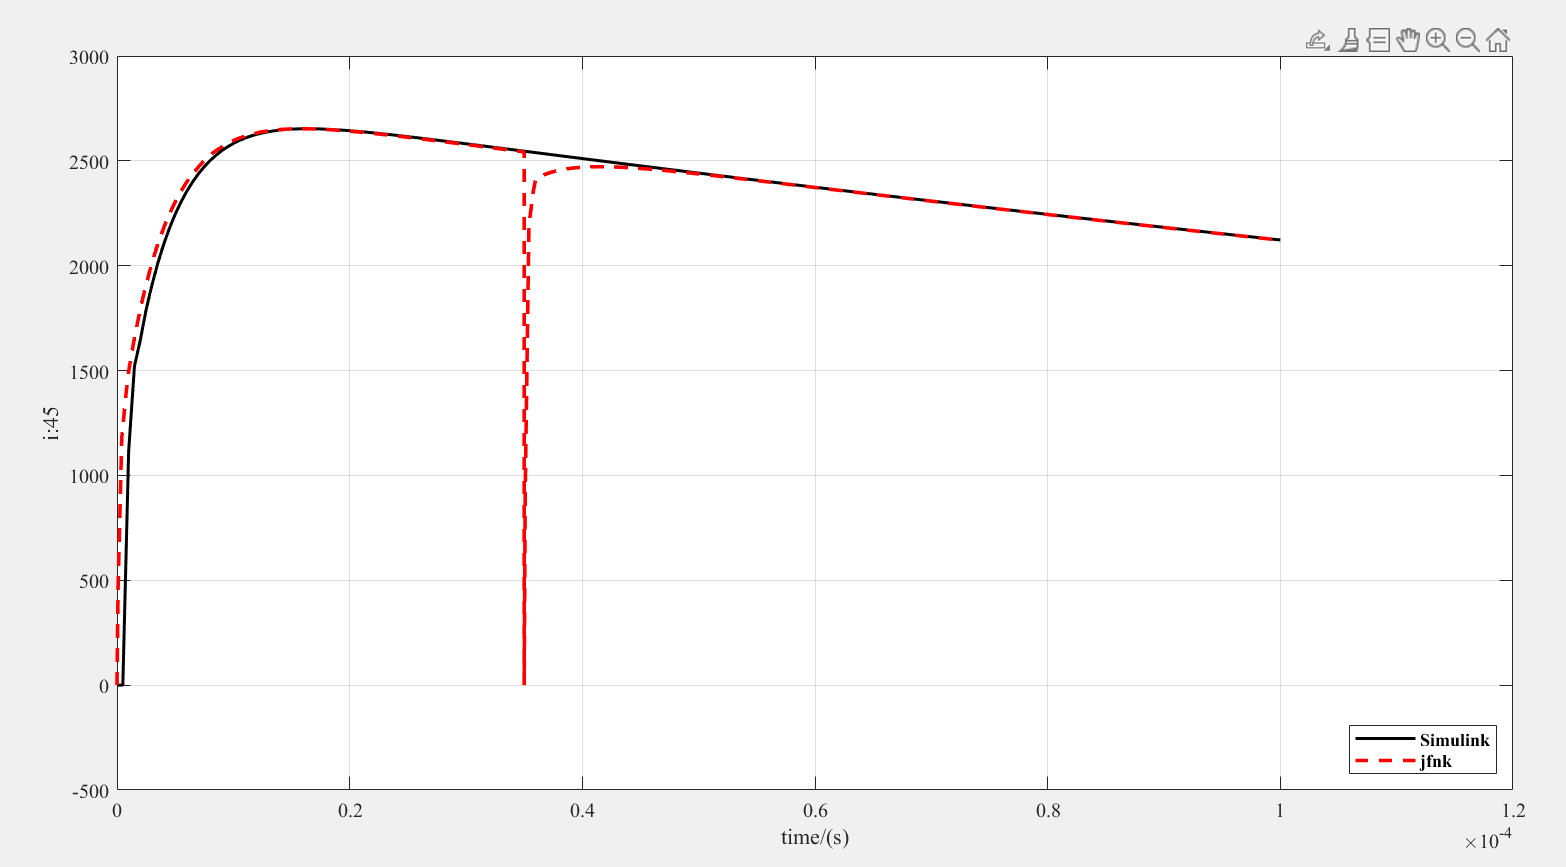
\includegraphics[width=0.8\textwidth]{45_jfnk.png}
    \caption{T6-IL (jfnk求解,N\_ITER\_MAX\_NEWTON = 50,N\_ITER\_MAX\_SDC = 100, t=[0,1e-4])}
    \label{fig:motor_structures}
\end{figure}
\indent JFNK运行时间: \newline
\indent  \text{JFNK\_onestep():  35.1653 s}
\indent  \text{save\_results():  0.0044 s}

\end{document}
